\setcounter{secnumdepth}{1}

\chapter{PID Controller}
\label{section:PID controller}

\section{Requirements analysis}

The first step of the controller design is to analyse the requirements that have been given in the introduction:

\begin{enumerate}
    \item[$\bullet$] the shaft can reach any reasonable speed in less than half a second
    \item[$\bullet$] the shaft's speed in maintained as smooth as possible
    \item[$\bullet$] the system can reject a step disturbance as fast as possible
    \item[$\bullet$] the shaft's speed can follow a feasible speed reference of $4 Hz$ from any feasible speed
\end{enumerate}

There is one reference tracking objective, one disturbance rejection objective and two dynamical response properties.
The design of the controller will follow the following path:

\begin{enumerate}
    \item Rejecting a step disturbance (with each motor separately)
    \item Following a $4 Hz$ reference (with each motor separately)
    \item Merge the two controllers into a single digital one
    \item Reach any speed in $< 0.5 s$
\end{enumerate}

The method used here is to design the controller in the Laplace domain in the first time. Once the continuous time
controller has the desired behaviour, it is discretized using the Tustin method (without forgetting to take the
ZOH into account).

\section{Disturbance rejection}

From theory, it is known that a controller is able to asymptotically reject a disturbance if it has at the denominator
of its transfer function the denominator of the disturbance.\\

As a step disturbance is of the form:

\begin{equation}
    D(s) = \frac{A e^{-\tau s}}{s}
\end{equation}

The controller will need a pole in $0$. This can be easily done by using a PI controller, which looks like:

\begin{align}
    C_{PI}(s) &= k_p \left( 1 + \frac{1}{T_i s} \right)\\
    &= k_p \left(\frac{T_i s + 1}{T_i s} \right)
    \label{eq:general_PI}
\end{align}

The $k_p$ will be chosen once the dynamic response characteristics will have to be met. However, $T_i$ can already be 
chosen based on a simple criteria. As the open-loop transfer function equals the product $C_{PI}(s) \times G_{1+} (s)$, a
solid choice is to use $T_i$ to cancel the pole in the system. This way, the position of the poles of the closed-loop
will be entirely based on the controller.\\
Of course this will be true in the case of a perfect model but as proved in the section \ref{section_validation}, the
parameter $\tau$ of the transfer function (which fixes the pole of it) does not seems to move a lot depending on the 
operating point. We can conclude from this that the best choice is:

\begin{equation}
    T_i = \tau
\end{equation}

for each controller, which leads to:

\begin{equation}
    C_{PI}(s) = k_p \left( \frac{\tau s + 1}{\tau s} \right) 
    \label{eq:controller_PI}
\end{equation}


\iffalse
\section{Reference tracking}

For tracking purposes, the method used to reject disturbances can also be applied. Indeed, a reference with $D(s)$ at
its denominator will be perfectly followed if the controller denominator contains $D(s)$.

\begin{align}
    R(s) &= \mathcal{L}\left\{A \sin (8 \pi t + \varphi)\right\} \\
    &= \frac{8 A \pi e^{-\frac{\varphi s}{8 \pi}}}{s^2 + (8\pi)^2}
\end{align}

A second controller is needed to ensure the tracking of a $4 Hz$ sine:

\begin{equation}
    C_{\sin}(s) = \frac{1}{s^2 + (8\pi)^2}
    \label{eq:controller_sin}
\end{equation}

This controller has no parameter that can be moved as we chose a minimalist controller. 
\fi

\section{Frequential analysis}
\label{section:freq_analysis}

As the next objective is to perfectly track a $4 Hz$ reference, the bandwidth of the closed loop has to be studied. If
it is greater than $4 \times 2\pi \approx 25$, then there is no need to add a part to the controller's structure.\\
The bandwidth is determined using the Bode curves of the closed loop. This means that the structure of the regulator
has to be defined. In continuous time, it looks like:

\begin{figure}[H]
    \centering
    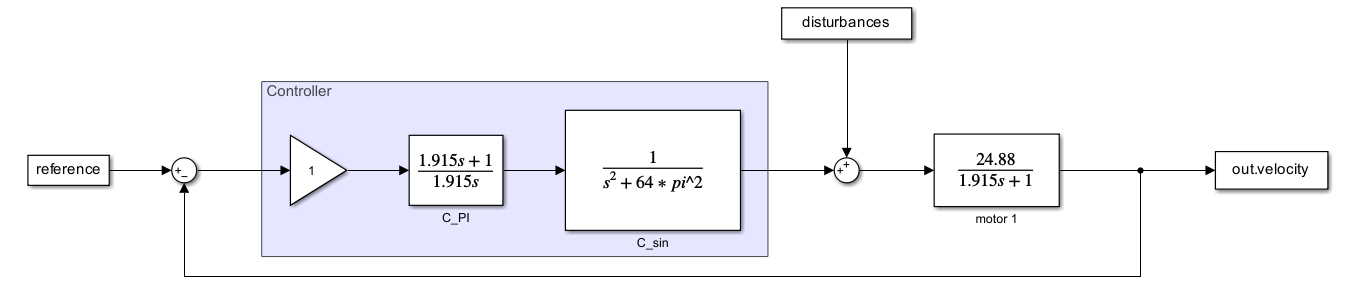
\includegraphics[height=\textheight/7]{Pictures/controller_structure.png}
    \caption{Structure of the closed loop system with a PI regulator}
    \label{fig:CL structure}
\end{figure}

To determine the gain (= $k_p$) that can be put in the system, the \texttt{margin} method of matlab is used (fig 
\ref{fig:OL bode}) on the open-loop transfer function with $k_p$ set to 1. A gain margin of $6 dB$ has to be maintained 
\footnote{by convention} to ensure the stability of the system once the loop is closed. \\

\begin{figure}[H]
    \centering
    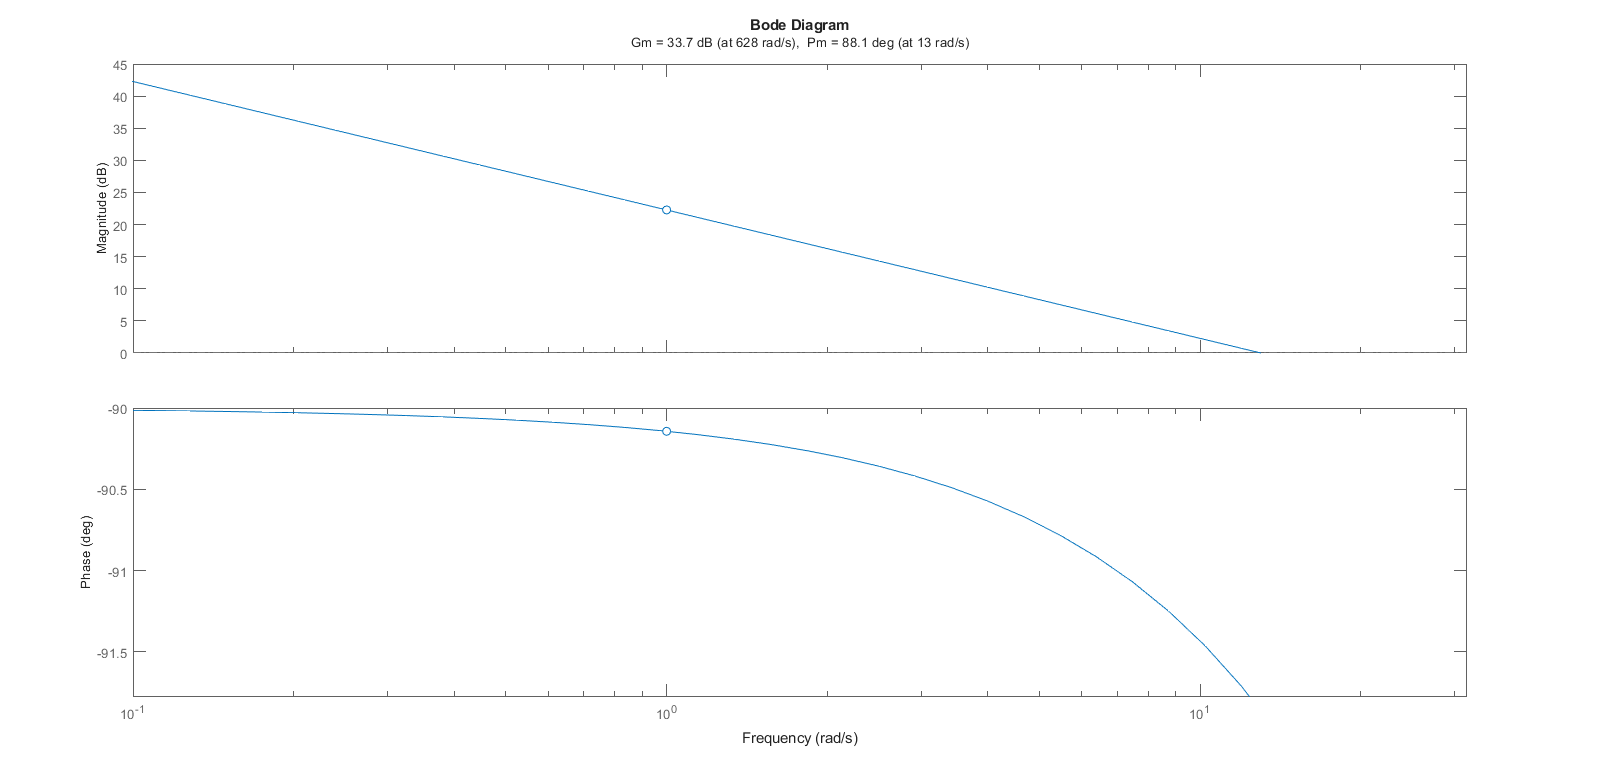
\includegraphics[height=\textheight/3]{Pictures/bode_OL.png}
    \caption{Bode diagram of the open loop system with the stability margins}
    \label{fig:OL bode}
\end{figure}

To keep a gain margin of at least $6 dB$, we can multiply $k_p$ (which was set to 1) by $27.7 dB = 10^{27.7/20} = 24.26$
. This means that if the loop is closed with $k_p = 24$, the closed loop system will be stable and it's bandwidth can
be determined. This is done by taking the frequency at which the gain of the closed loop system falls under $-3 dB$.\\ 
Figure \ref{fig:CL bode} gives a bandwidth of around $709 \text{rad}/s$. However to be more realistic and also to stay 
with a small phase (as it reaches $-200 ^{\circ}$ when the magnitude is $-3 dB$), the "\textit{safe}" bandwidth is $111 
\text{rad}/s$. This proves that a simple PI controller is sufficient to perfectly track a signal at $4 Hz$.

\begin{figure}[H]
    \centering
    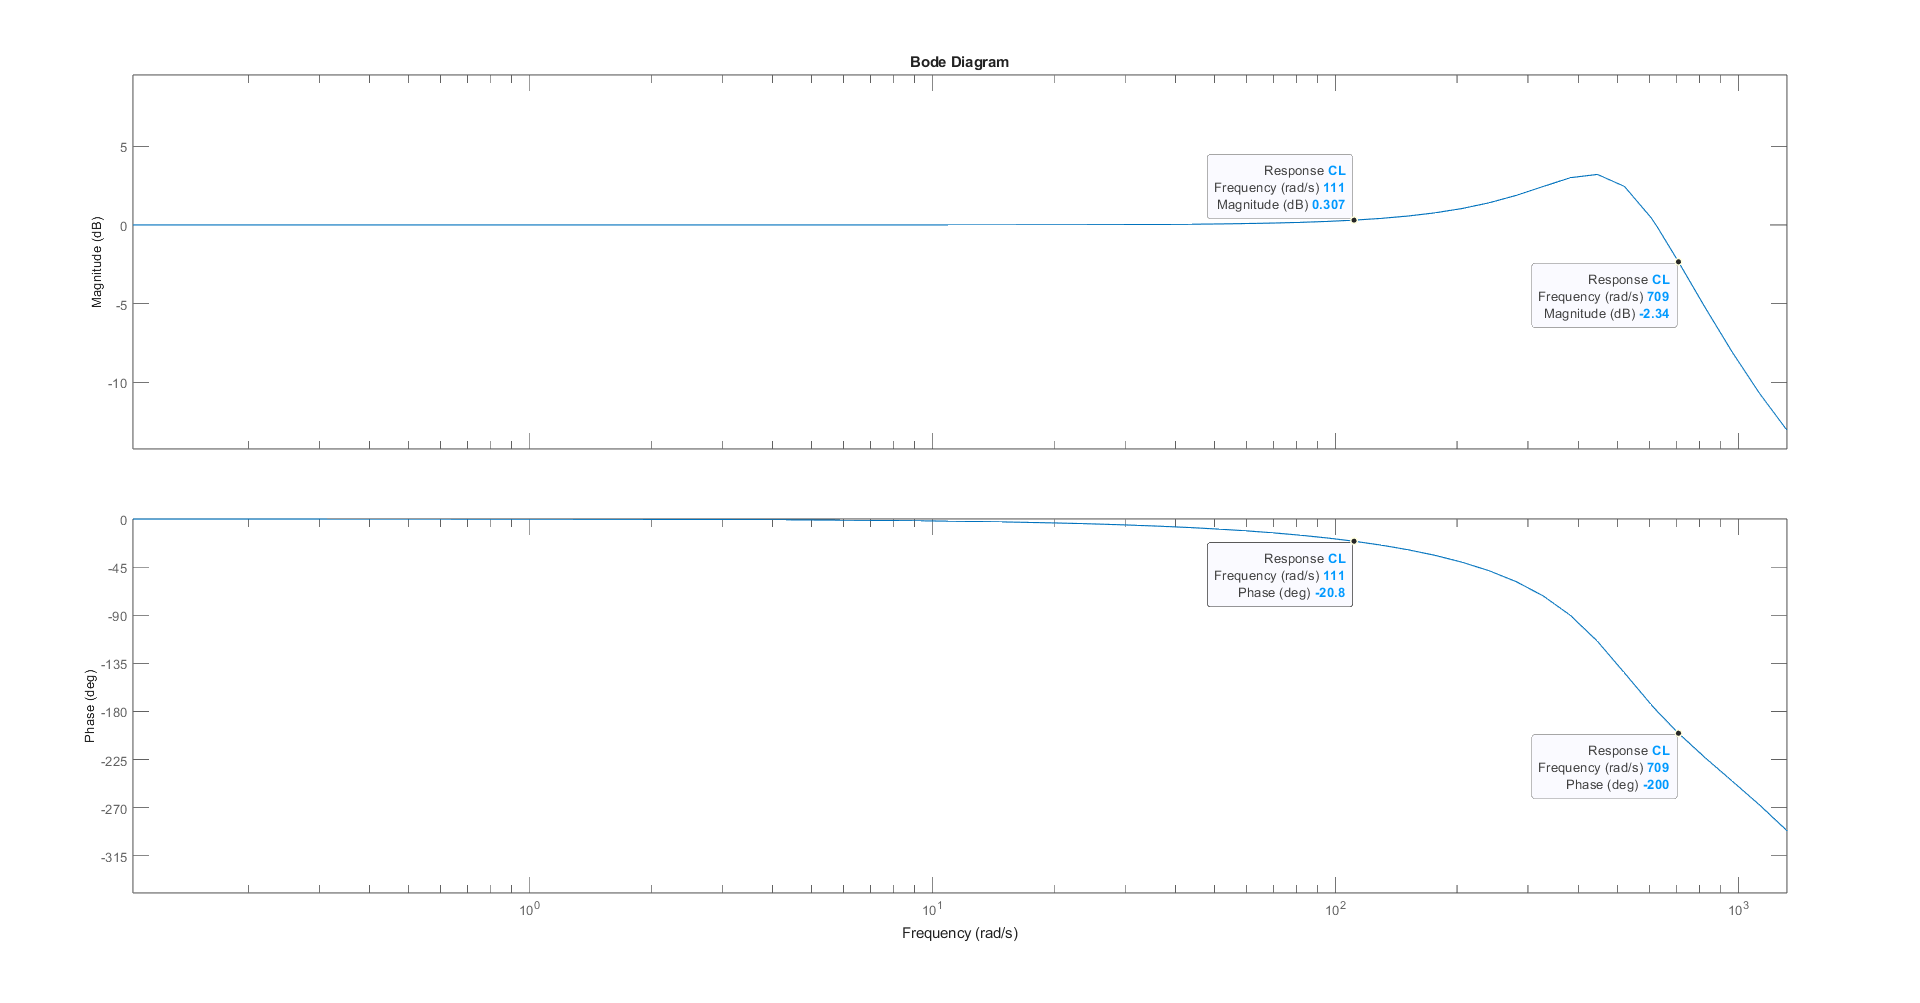
\includegraphics[height=\textheight/3]{Pictures/bode_CL.png}
    \caption{Bode diagram of the closed loop system for $k_p = 24$}
    \label{fig:CL bode}
\end{figure}

